% THIS IS SIGPROC-SP.TEX - VERSION 3.1
% WORKS WITH V3.2SP OF ACM_PROC_ARTICLE-SP.CLS
% APRIL 2009
%
% It is an example file showing how to use the 'acm_proc_article-sp.cls' V3.2SP
% LaTeX2e document class file for Conference Proceedings submissions.
% ----------------------------------------------------------------------------------------------------------------
% This .tex file (and associated .cls V3.2SP) *DOES NOT* produce:
%       1) The Permission Statement
%       2) The Conference (location) Info information
%       3) The Copyright Line with ACM data
%       4) Page numbering
% ---------------------------------------------------------------------------------------------------------------
% It is an example which *does* use the .bib file (from which the .bbl file
% is produced).
% REMEMBER HOWEVER: After having produced the .bbl file,
% and prior to final submission,
% you need to 'insert'  your .bbl file into your source .tex file so as to provide
% ONE 'self-contained' source file.
%
% Questions regarding SIGS should be sent to
% Adrienne Griscti ---> griscti@acm.org
%
% Questions/suggestions regarding the guidelines, .tex and .cls files, etc. to
% Gerald Murray ---> murray@hq.acm.org
%
% For tracking purposes - this is V3.1SP - APRIL 2009

\documentclass{acm_proc_article-sp}

\begin{document}

\title{PushUp: An event-based http Long-polling Server}
%
% You need the command \numberofauthors to handle the 'placement
% and alignment' of the authors beneath the title.
%
% For aesthetic reasons, we recommend 'three authors at a time'
% i.e. three 'name/affiliation blocks' be placed beneath the title.
%
% NOTE: You are NOT restricted in how many 'rows' of
% "name/affiliations" may appear. We just ask that you restrict
% the number of 'columns' to three.
%
% Because of the available 'opening page real-estate'
% we ask you to refrain from putting more than six authors
% (two rows with three columns) beneath the article title.
% More than six makes the first-page appear very cluttered indeed.
%
% Use the \alignauthor commands to handle the names
% and affiliations for an 'aesthetic maximum' of six authors.
% Add names, affiliations, addresses for
% the seventh etc. author(s) as the argument for the
% \additionalauthors command.
% These 'additional authors' will be output/set for you
% without further effort on your part as the last section in
% the body of your article BEFORE References or any Appendices.

\numberofauthors{2} %  in this sample file, there are a *total*
% of EIGHT authors. SIX appear on the 'first-page' (for formatting
% reasons) and the remaining two appear in the \additionalauthors section.
%
\author{
% You can go ahead and credit any number of authors here,
% e.g. one 'row of three' or two rows (consisting of one row of three
% and a second row of one, two or three).
%
% The command \alignauthor (no curly braces needed) should
% precede each author name, affiliation/snail-mail address and
% e-mail address. Additionally, tag each line of
% affiliation/address with \affaddr, and tag the
% e-mail address with \email.
%
% 1st. author
\alignauthor
Kai Liu \\
       \affaddr{Very Large Information System}\\
       \affaddr{Carnegie Mellon University}\\
       \email{hfevers@gmail.com}
% 2nd. author
\alignauthor
Yilun Cui \\
       \affaddr{Very Large Information System}\\
       \affaddr{Carnegie Mellon University}\\
       \email{yiluncui@gmail.com}
}
% There's nothing stopping you putting the seventh, eighth, etc.
% author on the opening page (as the 'third row') but we ask,
% for aesthetic reasons that you place these 'additional authors'
% in the \additional authors block, viz.

% Just remember to make sure that the TOTAL number of authors
% is the number that will appear on the first page PLUS the
% number that will appear in the \additionalauthors section.

\maketitle
\begin{abstract}
Traditionally, the http communication follows the pull model, where the client initiates the request and server responds it. However, for web pages that demand ``instant interaction'' between client/server or client/client, the pull model falls short because the frequent client-initiated communication will incur a huge overhead.

To overcome the problem, people proposed the ``long polling'' (also dubbed as ``comet''). With the long polling technology the http server will not terminate a connection after responded data has been delivered to a client; instead, the server will keep the connection alive so when new event occurs the server can send the updated message to the client immediately.

However this approach requires the server to keep a large amount of active connections. To efficiently manage the connections we proposed to add an event-based reverse proxy server in between of client and backend servers. So when a new client/server session is established, the reverse will (1) keep the the connection open, and (2) retrieves resources on behalf of a client from backend servers. Meanwhile the backend servers can send the updates to the proxy server and the proxy server
will propagate the updates to related active clients.

We plan to benchmark our reverse proxy software with Twitter stream-like applications which will constantly be publishing new feeds to a large number of subscribers. We will compare the performance of the reverse proxy with the traditional opening and closing connection to evaluate the strengths and weaknesses of our approach. 
\end{abstract}

\section {Introduction\\}
Traditionally, the web server is a classical example of the request/response 
model, where the clients can retrieve the resource from the server but the 
server cannot push the data to the client actively. 

However, with the increasing popularity of Ajax\cite{Ajax} technologies, there 
are many scenarios where servers would like to actively notify the clients the 
latest updates. For example, the new messages in chat room, latest tweets in 
twitter, etc.

To overcome the limitation of request/response model, many approaches has been 
proposed to build more responsive sites. For example:

\begin{itemize}
\item Client Pull: the client sends update requests periodically to pull the
updates from server. This method is very easy to implement because 
it is stateless and the web server doesn't need to put much effort to modify 
its architecture. However, client pull will generate lots of http requests.
The work flow of client pull is illustrated in Figure \ref{fig:client_pull}.

\item Plugins: since the HTTP itself doesn't provide any mechanism for server 
push, plugins, such as the Flash, Silverlight, Javelet, etc, can be used as an 
extension of the HTTP by providing more flexible client/server communication 
mechanisms. However plugins is non-standard and requires users' extra effort to 
install and configure them.
\end{itemize}

Given those drawbacks, we focus on the another solution: long polling
\cite{LongPolling}. The work flow of long polling can be described in Figure
\ref{fig:long_polling}. When a client ``asks for"(polls) an update by sending 
an HTTP request to the server, if the no information is yet available, the 
server will not terminate the connection immediately; Instead, the server 
will keep the connection open for a period of time until (1) the information 
become available (2) after a suitable timeout($50$ seconds is a common choice).

The benefit to long-polling is that there is less back-and-forth between the 
client and server. The server is in control of the timing, so updates to the
browser can be made within milliseconds. This makes it ideal for some highly
interactive web applications.

\begin{figure}[htb!]
\centering
    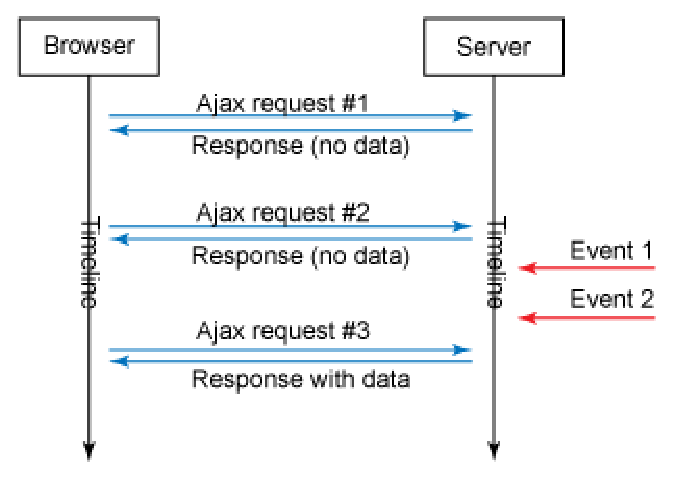
\includegraphics[scale=0.70]{figures/client_pull.eps}
    \caption{Client Pull Work Flow}
    \label{fig:client_pull}
\end{figure}

\begin{figure}[htb!]
    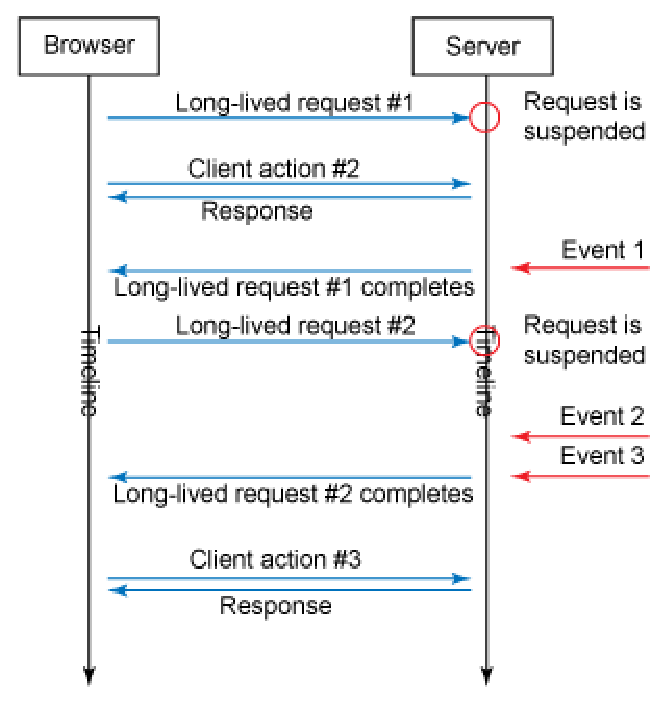
\includegraphics[scale=0.70]{figures/long_polling.eps}
    \caption{Long Polling Work Flow}
    \label{fig:long_polling}
\end{figure}

The down-side of long polling is that the server may have to deal with large
number of active connections between the clients and the servers. For example,
if you have one million users and, 10\% of them will be online. In this case,
the server should be able to hold at least 100,000 concurrent connections.

To address these problems, we present the event-based\cite{UnixBook}, scalable
long polling server PushUp to provide dedicated long polling services for 
different web applications with less resource cost.

As illustrated in Figure \ref{fig:sim_pushup}, the PushUp server lies in 
between of clients and web servers. It has two main responsibilities:
\begin{figure}[htb!]
\centering
    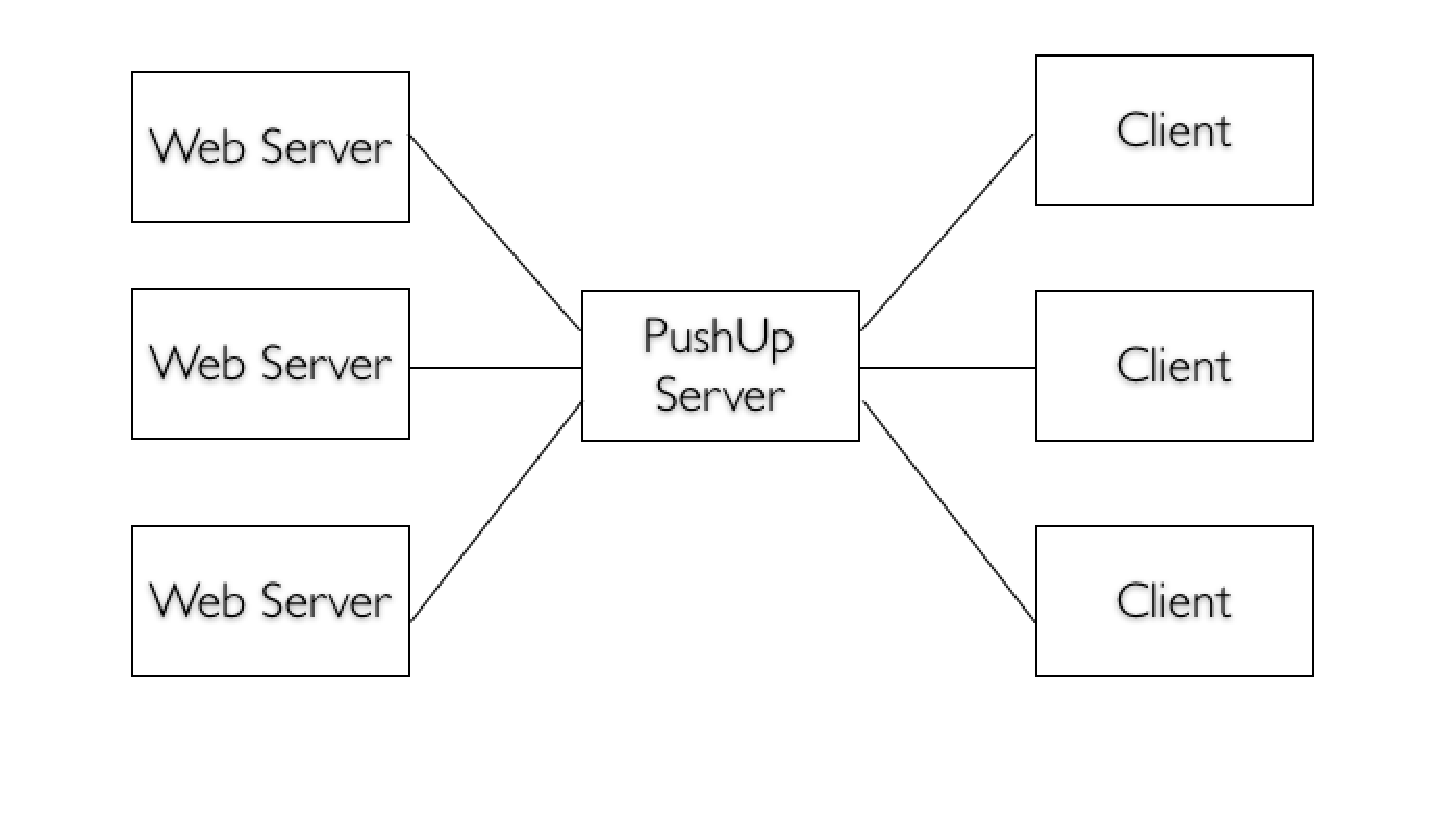
\includegraphics[scale=0.40]{figures/sim_pushup.eps}
    \caption{Simplified Architecture of the PushUp}
    \label{fig:sim_pushup}
\end{figure}

\begin {itemize}
\item {\bf An event-based message queue}\cite{PubSub} to provide the long 
polling services. It keeps the active connections with very low overhead.
The core to this component is an event-based message queue provides
publication interface for the web servers and the subscription interface
for the clients.
\item {\bf An event-based reverse proxy}\cite{ReverseProxy} that retrieves 
resources on behalf of a client from one or more servers.
\end {itemize}

The message queue and reverse proxy of PushUp server forms an intermediary
between browsers and web servers. When a client request arrives the PushUp
will forward non-update-polling to the backend web servers and the long 
polling requests to the message queues. Doing this allows both clients and
web servers work with minimal awareness of PushUp Server. 

\section{Related Work\\}

\subsection{Event vs. Thread\\}

Some stuff mentioned in the class.

\subsection{Server Push technologies\\}

In \cite{Engin}, Bozdag \emph{et al} provided a complete comparison 
and evaluation of different server push technologies, including the 
HTTP pull, Flash XML socket, Java RMI, etc. As a conclusion the authors 
stated that "an event-driven model on the server side is necessary" 
owing to its , lower consumption of the computing resource, less network
traffic etc.

Another paper \cite{duquennoy09consistency} performs the quantitative 
analysis of the consistency and scalability of several different server
push technologies. As the experimental results showed the event-driven
long polling model shows an excellent efficiency and scalability.


\section {Evaluation\\}

In this section, we conducted experiments to evaluate the performance of 
three web-based message delivery mechanisms. 

\begin{itemize}
    \item {\bf Client Pulling (CP): } In this model the client side initiates 
        an http request to the server to pull the latest updates on a regular 
        basis.
    \item {\bf Multithreadeding long polling(MLP): } This model realizes the 
        long polling by multi threads. For each incoming polling request, the
        server will create a thread waiting for the latest updates.
    \item {\bf Event-based long polling(ELP): } This model realizes the long
        polling by event-based mechanism. This model keeps all the polling 
        requests within a single thread.
\end{itemize}

\subsection{Settings \\}

\subsubsection{Evaluation Metrics \\}
In the evaluation, we used the following control variables to control in
the experiments.

\begin{itemize}
    \item {\bf Number of concurrent connections}: This variable allows us 
         to evaluate the scalability of different methods.
    \item {\bf Publish Interval}: This variable controls the frequency of 
         event publication by the server. 
    \item {\bf Polling interval}: This variable determines how long will 
        the method send a polling request to the server. For client 
        pulling, it sends polling request at a regular basis; as for
        long polling methods, they send polling request (1) after they
        just received a new update or (2) after a suitable timeout.
\end{itemize}

And we used the following metrics to evaluate the performance of different
methods.
\begin{itemize}
    \item {\bf Network Traffic (NT)}: NT evaluates the network usage for
        different event notification methods.
    \item {\bf Mean Publish Trip Time (MPT)}: The publish trip-time is 
        the time elapsed between the creation of a data by the server and 
        its reception by the client. It shows how long it takes for the 
        client to be updated when an event occurs.
    \item {\bf Received Message Percentage (RMP)}: RMP indicates the data 
        loss in during the network communication. 
    \item {\bf Server Memory Usage (SMU)}: In many real world long polling 
        system, the polling requests spent most of their time waiting for 
        the new events.[source needed] Thus, memory cost for each idle 
        polling requests is critical to the overall performance.
\end{itemize}

\subsubsection{Evaluation Environment \\}
The experiments are done in CMU's PEACE cluster. Each machine in the cluster 
has a 4 CPU cores(AMD Opteron Processor 4130, 2600 MHz, 512K cache size),
8 GB RAM and 1 physical 581 GB disk.

\subsection{Push Model vs. Poll Model\\}

One of the biggest advantage of long polling strategy is its significant 
reduction of network traffic. In the following experiments we focused on
the evaluation on the network traffic(NT) and mean publish trip time(MPT).

Since the goal of these experiments is to characterize the network traffic 
of different models. We evaluated the {\bf network traffic} and {\bf mean 
publish trip time} only with some moderate number of concurrent 
connections: 10, 100 and 1000. 

The {\bf publish time} are $10 sec$, $20 sec$, $30 sec$, $40 sec$ and 
$50 sec$. The {\bf polling time} we chose for the {\bf client pulling}
is $1 sec$, and $50 sec$ for long polling based models(which is a 
popular choice in real world long polling applications).

Table \ref{tb:traffic} shows the detailed network traffic with different 
publish time and number of concurrent connections (written as "cc" 
in the tables).  We can see that the long polling based model keeps 
a relatively constant network traffic while the client pull model's 
network traffic grows (almost) linearly as the publish time increases.
Figure \ref{fig:traffic} shows the network traffic change when the number 
of concurrent connection is $1000$.

Table \ref{tb:mpt_all} demonstrates the mean publish trip time with 
different publish time and number of concurrent connections. The MPT of
client pull increases much faster than the long polling based models.
This may because the growing network traffic increases the chance
of package loss in the client pull model. 
Figure \ref{fig:traffic_latency} compares the MPT of push and pull models when 
the number of concurrent connection is $1000$.

In summary, the push model significantly reduce the network traffic, which in
turn, yields a smaller mean publish trip time as the concurrent connections 
increase. 

Also, we observed that the multithreading-based long polling and event-based long 
polling have similar performance in terms of network traffic and mean publish
trip time when the number of concurrent connections is relatively small. In the 
following next we will test both long polling models' performance with large 
concurrent connections.

\begin{table}
\centering \caption{\label{tb:traffic} Network Traffic(KB)}
\begin{tabular}{|l|l|l|l|l|l|}
    \hline cc=10& 10 sec & 20 sec & 30 sec & 40 sec & 50 sec \\
    \hline CP & 12.7 & 25.8 & 39.8 & 55.2 & 68.2 \\
    \hline MLP & 1.27 & 1.27 & 1.27 & 1.27 & 1.27 \\
    \hline ELP & 1.27 & 1.27 & 1.27 & 1.27 & 1.27 \\
    \hline
    \hline cc=100& 10 sec & 20 sec & 30 sec & 40 sec & 50 sec \\
    \hline CP & 127.4 & 277.1 & 415.2 & 580.5 & 745.5 \\
    \hline MLP & 12.7 & 12.7 & 12.7 & 12.7 & 13.1 \\
    \hline ELP & 12.7 & 12.7 & 12.7 & 12.7 & 12.7 \\
    \hline
    \hline cc=1000 & 10 sec & 20 sec & 30 sec & 40 sec & 50 sec \\
    \hline CP & 1370.5 & 3457.1 & 5537.5 & 7282.5 & 10743.5 \\
    \hline MLP & 135.5 & 132.5 & 137.8 & 133.4 & 135.5 \\
    \hline ELP & 130.1 & 129.5 & 132.8 & 131.8 & 130.5 \\
    \hline
\end{tabular}
\end{table}

\begin{figure}[htb!]
\centering%
    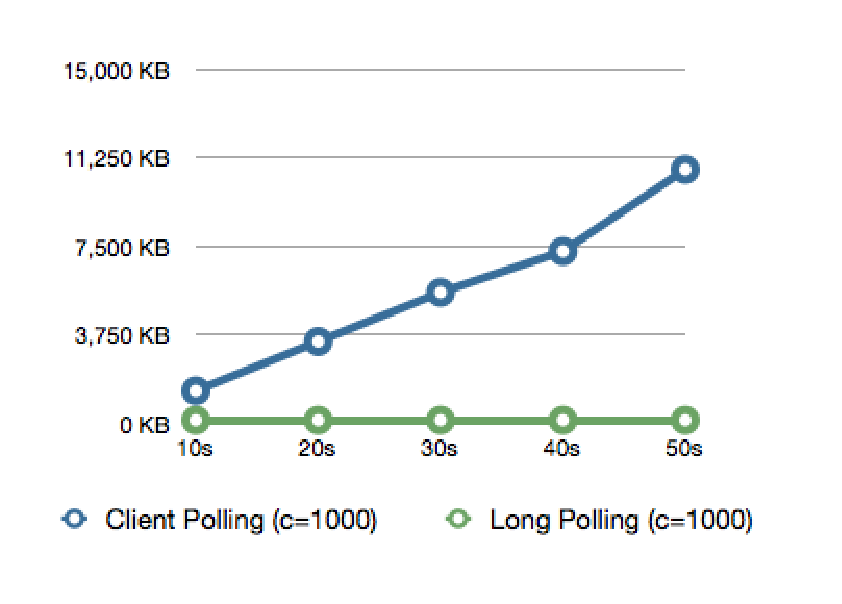
\includegraphics[scale=0.60]{figures/io.eps}
    \caption{Network Traffic of Pull \& Push Models}
    \label{fig:traffic}
\end{figure}


\begin{table}
\centering \caption{\label{tb:mpt_all} Mean Publish Trip Time (second)}
\begin{tabular}{|l|l|l|l|l|l|}
    \hline cc=10 & 10 sec & 20 sec & 30 sec & 40 sec & 50 sec \\
    \hline CP & 0.6 & 0.7 & 0.5 & 0.7 & 0.8 \\
    \hline MLP & 0.1 & 0.0 & 0.1 & 0.2 & 0.1 \\
    \hline ELP & 0.2 & 0.1 & 0.1 & 0.4 & 0.2 \\
    \hline
    \hline cc=100 & 10 sec & 20 sec & 30 sec & 40 sec & 50 sec \\
    \hline CP & 0.8 & 1.1 & 2.5 & 3.1 & 2.7 \\
    \hline MLP & 0.5 & 0.4 & 0.5 & 0.8 & 1.1 \\
    \hline ELP & 0.7 & 0.4 & 0.8 & 1.2 & 0.9 \\
    \hline
    \hline cc=1000& 10 sec & 20 sec & 30 sec & 40 sec & 50 sec \\
    \hline CP & 2.8 & 3.4 & 4.5 & 5.3 & 7.2 \\
    \hline MLP & 2.3 & 2.9 & 2.7 & 3.5 & 3.4 \\
    \hline ELP & 2.4 & 2.8 & 1.8 & 2.4 & 2.9 \\
    \hline
\end{tabular}
\end{table}

\begin{figure}[htb!]
\centering%
    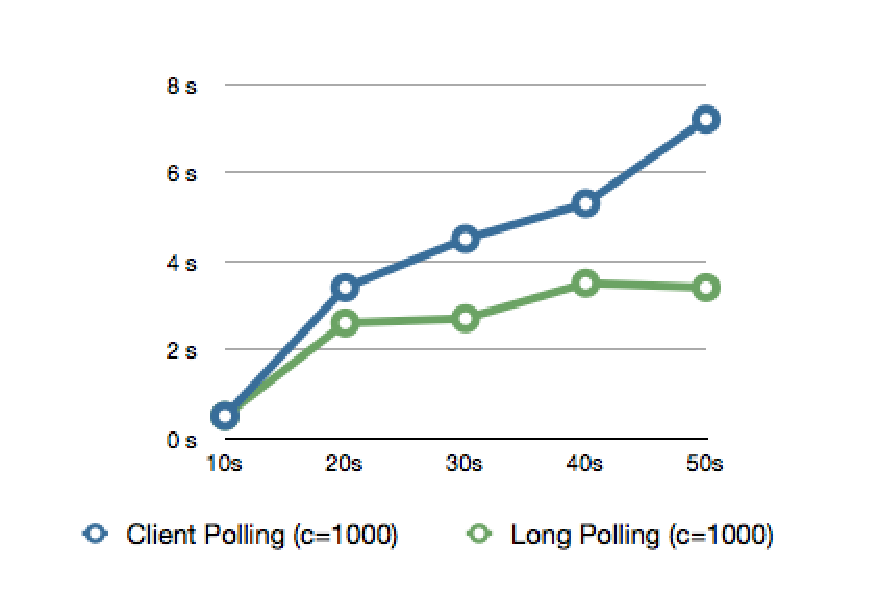
\includegraphics[scale=0.60]{figures/latency.eps}
    \caption{Mean Publish Trip Time of Pull \& Push Models}
    \label{fig:traffic_latency}
\end{figure}

\subsection{Event vs. Thread\\}

Here we compared the performance between event-based long polling model
and the multithreading long polling model. In the following evaluation
we tested the {server memory usage(SMU)}, {\bf mean publish trip time
(MPT)}, {\bf received message percentage(RMP)} with large number of
active connections(from 500-16000).

Figure \ref{fig:et_memory} shows the server memory usage of both models.
The event-based model demonstrates an excellent memory usage as the
number of active connections increases, while the memory usage of 
multithreading model soars rapidly and reaches $100\%$ when the active
connections' number goes to $8000$.

Figure \ref{fig:et_latency} and figure \ref{fig:et_rate}, show the mean
publish trip time and received message percentage. Event-based model 
significantly excels multithreading model in both evaluation.

Thus we claimed multithreading approach is not a good choice as its
memory usage and possible context switch may incur very large overhead,
which heavily lowered the system performance. The event-based mode, on
the other hand, demonstrates a slower performance decrease as the
number of concurrent connections increases.

\begin{figure}[htb!]
\centering%
    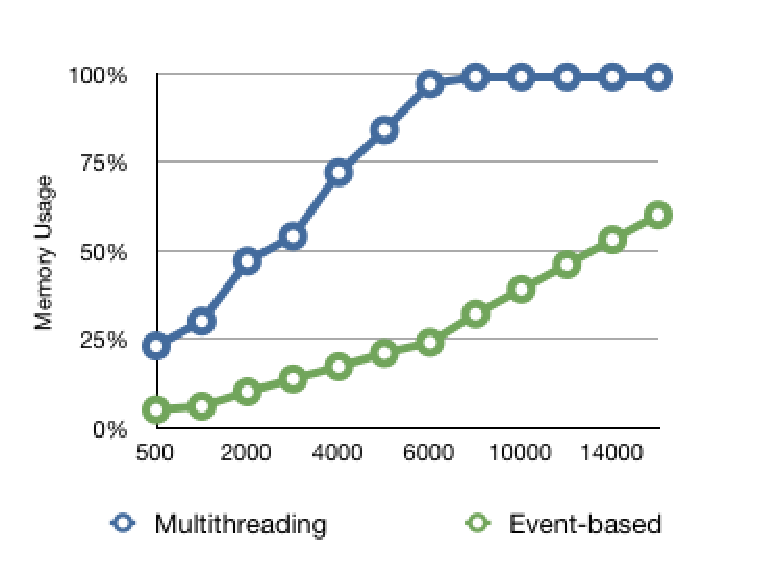
\includegraphics[scale=0.70]{figures/et_memory.eps}
    \caption{Server Memory Usage}
    \label{fig:et_memory}
\end{figure}

\begin{figure}[htb!]
\centering%
    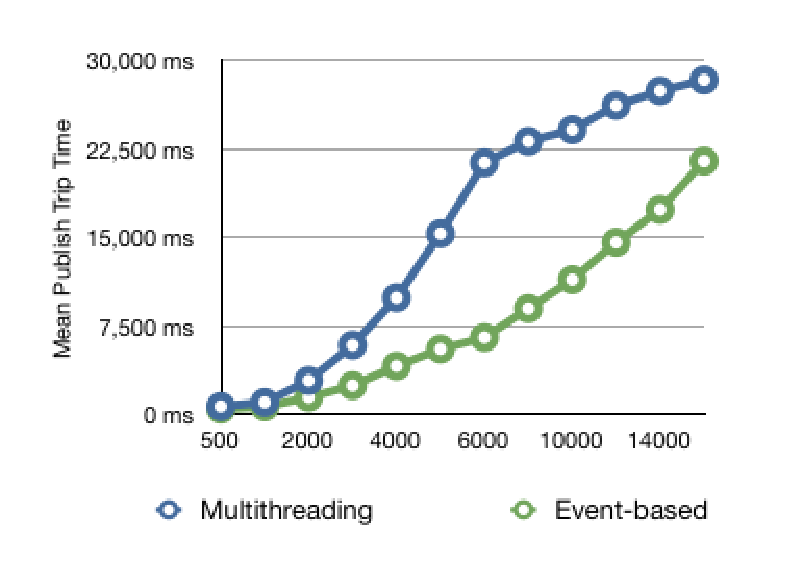
\includegraphics[scale=0.70]{figures/et_latency.eps}
    \caption{Mean Publish Trip Time}
    \label{fig:et_latency}
\end{figure}

\begin{figure}[htb!]
\centering%
    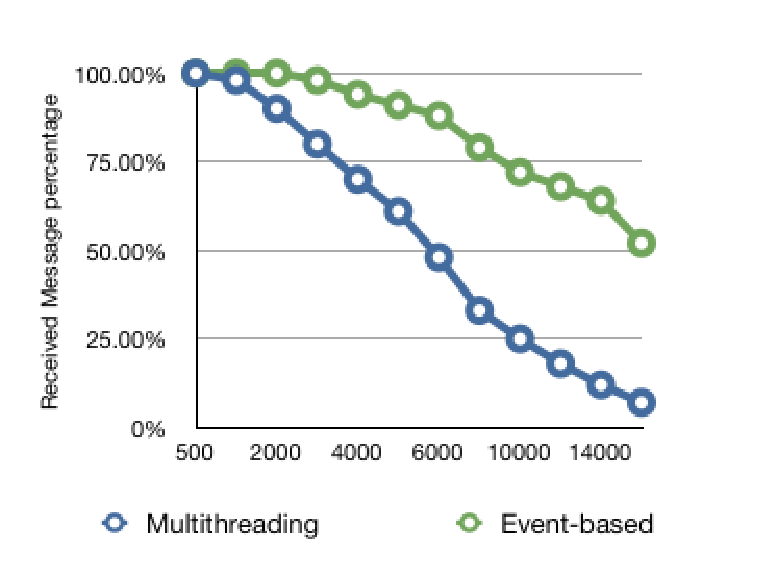
\includegraphics[scale=0.70]{figures/et_rate.eps}
    \caption{Received Message Percentage}
    \label{fig:et_rate}
\end{figure}


\subsection{Extending PushUp Server\\}

* Design goal: Comparison between different models, what are the expected experimental results.

* How do you conduct the experiment?

* What is the exp results?

* Experiment analysis: What can you see from the experiment results? Does it match your expectation?


How they can serve large amount of active connection.

Metrics:

Up to 20000 connections.

HAProxy, very simple load balancing.

1, 2, 3, 4, 5

The Load balance create a little overhead (how much?).

But overall the overhead is acceptable.




\subsection{Measuring the Active Connections\\}



%
% The following two commands are all you need in the
% initial runs of your .tex file to
% produce the bibliography for the citations in your paper.
\bibliographystyle{abbrv}
\bibliography{sigproc}  % sigproc.bib is the name of the Bibliography in this case
% You must have a proper ".bib" file
%  and remember to run:
% latex bibtex latex latex
% to resolve all references
%
% ACM needs 'a single self-contained file'!
%
%APPENDICES are optional
%\balancecolumns
% That's all folks!
\end{document}
